\section{Theory}

\begin{frame}
        \centering
        \huge Theory
        \note{
                \begin{itemize}
                	\item Twitter Sentiment Analysis
                    \item Kappa
                    \item Multinomial Naive Bayes
                    \item Stochastic Gradient Descent
                \end{itemize}
                }
\end{frame}

\begin{frame}
	\frametitle{Twitter Sentiment Analysis}
	\begin{block}{Tweet Example}
		After a whole 5 hours away from work, I get to go back again, I’m so lucky!
	\end{block}
	\begin{itemize}
		\item Need labeled data
		\item Emoticons as indicators of sentiment
		\begin{itemize}
			\item Negative Sentiment - :(
			\item Positive Sentiment - :)
		\end{itemize}
	\end{itemize}
\end{frame}

\begin{frame}
	\frametitle{Unbalanced Classes}
	\begin{table}[htb]
		\centering
		\begin{tabular}{llll}
			\multicolumn{1}{c}{} & Predicted Class+ & Predicted Class- & Total \\ \cmidrule{2-4}
			Correct Class+	& \num{75}	& \num{8}	& 83\\
			Correct Class-	& \num{7}	& \num{10}	& 17\\ \cmidrule{1-4}
			Total			& 82		& 18		& 100
		\end{tabular}
		\caption{Confusion matrix for hypothetical classifier}
	\end{table}

	\begin{table}[htb]
		\centering
		\begin{tabular}{llll}
			\multicolumn{1}{c}{} & Predicted Class+ & Predicted Class- & Total \\ \cmidrule{2-4}
			Correct Class+	& \num{68.06}	& \num{14.94}	& 83\\
			Correct Class-	& \num{13.94}	& \num{3.06}	& 17\\ \cmidrule{1-4}
			Total			& 82		& 18		& 100
		\end{tabular}
		\caption{Confusion matrix for chance predictor}
	\end{table}
	\note{$(75+7)*(75+8)/100 = 68.06$}
\end{frame}

\begin{frame}
	\frametitle{Kappa statistic}
	\begin{columns}
		\begin{column}{0.5\textwidth}
			\begin{itemize}
				\item Kappa is 0 or less if there is no agreement between the classifiers other than chance
				\item Kappa is 1 when the classifiers are in complete agreement
			\end{itemize}
		\end{column}
		\begin{column}{0.5\textwidth}  %%<--- here
			\begin{block}{Cohen's Kappa}
				\centering
				$\kappa = \frac{p_o-p_e}{1-p_e} = 1-\frac{1-p_o}{1-p_e}$
			\end{block}
			\begin{block}{Observed Accuracy}
				\centering
				$p_o = \frac{\sum_{i=l}^{L}C_{ii}}{m}$
			\end{block}
			\begin{block}{Expected Accuracy}
				\centering
				$p_c=\sum_{i=l}^{L}(\sum_{j=l}^{L}\frac{C_{ij}}{m}\times\sum_{j=l}^{L}\frac{C_{ji}}{m})$
			\end{block}
		\end{column}
	\end{columns}
	\note{
		\begin{itemize}
			\item observed proportionate agreement is $p_o$
			\item Normalizes the accuracy as a comparison of how much better the classifier is compared to a chance predictor
		\end{itemize}
	}
\end{frame}

\begin{frame}
	\begin{table}[htb]
		\centering
		\begin{tabular}{llll}
			\multicolumn{1}{c}{} & Predicted Class+ & Predicted Class- & Total \\ \cmidrule{2-4}
			Correct Class+	& \num{75}	& \num{8}	& 83\\
			Correct Class-	& \num{7}	& \num{10}	& 17\\ \cmidrule{1-4}
			Total			& 82		& 18		& 100
		\end{tabular}
		\caption{Confusion matrix for hypothetical classifier}
	\end{table}
	\begin{block}{Observed Accuracy}
		\centering
		$p_o = \frac{\sum_{i=l}^{L}C_{ii}}{m}$
	\end{block}
	\begin{block}{}
		\centering
		$p_o = \frac{75+10}{100} = 0.85$
	\end{block}
	\note{}
\end{frame}

\begin{frame}
	\begin{table}[htb]
		\centering
		\begin{tabular}{llll}
			\multicolumn{1}{c}{} & Predicted Class+ & Predicted Class- & Total \\ \cmidrule{2-4}
			Correct Class+	& \num{75}	& \num{8}	& 83\\
			Correct Class-	& \num{7}	& \num{10}	& 17\\ \cmidrule{1-4}
			Total			& 82		& 18		& 100
		\end{tabular}
		\caption{Confusion matrix for hypothetical classifier}
	\end{table}	
	\begin{columns}
		\begin{column}{0.5\textwidth}
			\begin{block}{Class+ Accuracy}
				\centering
				$\frac{(75+7)\times(75+8)}{100} = 68.06$
			\end{block}
		\end{column}
		\begin{column}{0.5\textwidth}  %%<--- here
			\begin{block}{Class- Accuracy}
				\centering
				$\frac{(10+7)\times(8+10)}{100} = 3.06$
			\end{block}
		\end{column}
	\end{columns}
	\begin{block}{Expected Accuracy}
		\centering
		$p_e = \frac{68.06+3.06}{100} = 0.7112$
	\end{block}
\note{
	
}
\end{frame}

\begin{frame}
	
	\begin{columns}
		\begin{column}{0.5\textwidth}
			\begin{itemize}
				\item $p_o = 0.85$
				\item $p_e = 0.7112$
			\end{itemize}
		\end{column}
		\begin{column}{0.5\textwidth}  %%<--- here
			\begin{block}{Cohen's Kappa}
				\centering
				$\kappa = \frac{p_o-p_e}{1-p_e} = 1-\frac{1-p_o}{1-p_e}$
			\end{block}
		\end{column}
	\end{columns}
	
	\begin{block}{Kappa}
		\centering
		$\kappa = \frac{0.85-0.7112}{1-0.7112} \approx 0.48$
	\end{block}
\end{frame}

\begin{frame}
	\frametitle{Sliding Window}
	\begin{itemize}
		\item Data stream changes over time
		\item Forgetting mechanism
		\item Kappa Sliding Windows Statistic
	\end{itemize}
	\begin{figure}
		\centering
		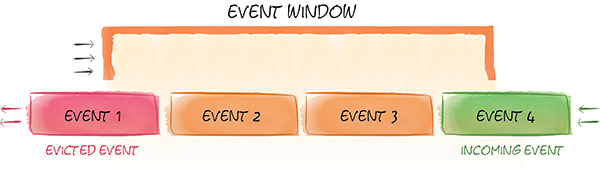
\includegraphics[scale=0.3]{slidingwindow.png}
	\end{figure}
\end{frame}

\begin{frame}
	\frametitle{Data Stream Mining Methods}
	\begin{itemize}
		\item Multinomial Naïve Bayes
		\item Stochastic Gradient Descent
		\item Hoeffding Tree
	\end{itemize}
\end{frame}

\begin{frame}
	\frametitle{Multinomial Naïve Bayes}
\begin{columns}
	\begin{column}{0.3\textwidth}
		\begin{itemize}
			\item bag of words
			\item Laplace correction
		\end{itemize}
	\end{column}
	\begin{column}{0.7\textwidth}  %%<--- here
		\begin{figure}
			\centering
			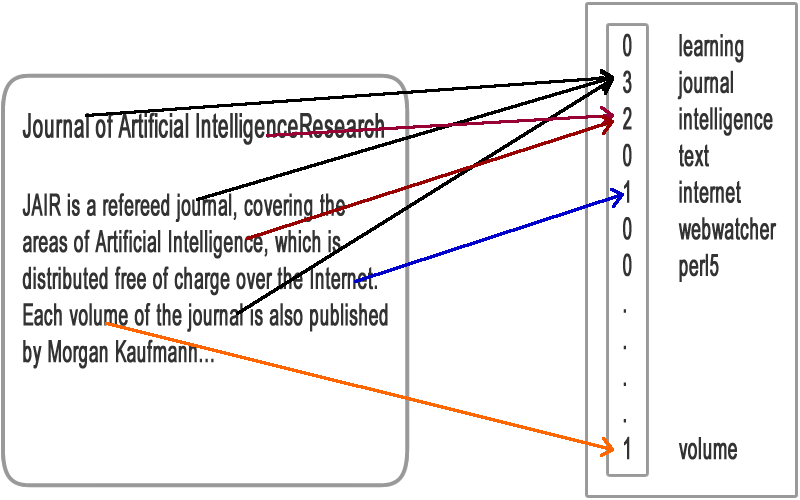
\includegraphics[scale=0.3]{bagofwords.png}
		\end{figure}
	\end{column}
\end{columns}


	\begin{block}{Probability of Class c}
		\centering
		$P(c|d) = \frac{P(c) \prod_{w\in d}P(w|c)^{n_{wd}}}{P(d)}$
	\end{block}
\note{To avoid the zero-frequency problem, it is
	common to use the Laplace correction for all conditional probabilities involved,
	which means all counts are initialized to value one instead of zero.
}
\end{frame}

\begin{frame}
	\frametitle{Stochastic Gradient Descent}
	\begin{columns}
		\begin{column}{0.5\textwidth}
			\begin{itemize}
				\item Vanilla Stochastic Gradient Descent
				\item Fixed learning rate
			\end{itemize}
		\end{column}
		\begin{column}{0.5\textwidth}  %%<--- here
			\begin{figure}
				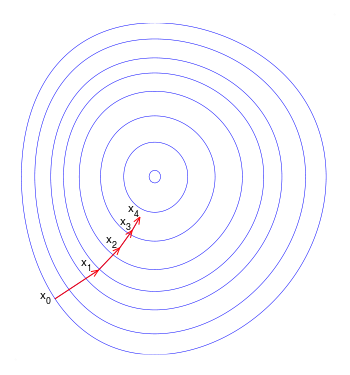
\includegraphics[scale=0.2]{gradientdescent.png}
			\end{figure}
		\end{column}
	\end{columns}
	
	\begin{block}{Loss Function}
		\centering
		$\frac{\lambda}{2}|w|^2+\sum[1-(yxw+b)]_+$
	\end{block}
	\note{
		\begin{itemize}
			\item w - weight vector
			\item b - bias
			\item $\lambda$ regularization parameter $ = 0.0001$
			\item y - class label, -1 to 1
			\item learning rate per example = 0.1 - too sow and it wouldn't adapt to changes in stream
		\end{itemize}
	}
\end{frame}

\begin{frame}
	\frametitle{Hoeffding Tree}
	\begin{columns}
		\begin{column}{0.5\textwidth}
			\begin{itemize}
				\item Pre-prune strategy based on the Hoeffding bound
				\item Uncommon for document classification
				\item Incrementally grows a decision tree
			\end{itemize}
		\end{column}
		\begin{column}{0.5\textwidth}  %%<--- here
			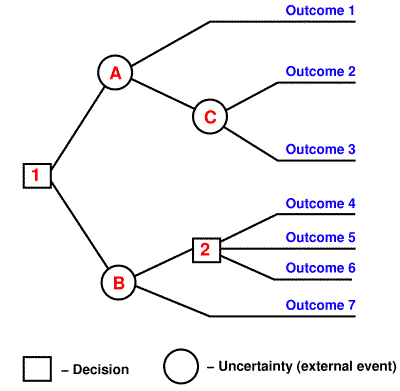
\includegraphics[scale=0.3]{decisiontree.png}
		\end{column}
	\end{columns}
	\begin{block}{Hoeffding Bound}
		\centering
		$\epsilon = \sqrt{\frac{R^2ln(1/\delta)}{2n}}$
	\end{block}
	\note{
		\begin{itemize}
			\item $\epsilon$ is the error on the node. R is the range random variable r. n is the number of observations.
			\item Each node tests an attribute
			\item Each branch is the outcome of that test
			\item Each leaf holds a class label
			\item For each training input - keep building till enough info, then split
		\end{itemize}
	}
\end{frame}